%% \frame{Theory (10 min)
%%   \begin{itemize}
%%   \item basics of nuclear physics and reactions
%%   \item neutron capture processes
%%   \item stellar evolution and galactic enrichment
%%   \item Omega
%%   \item Eris
%%   \end{itemize}
%% }

%% \frame{\comment{Nuclear physics} \\ atom + chart of nuclides \\ shell-model \\ reaction rates + \betadecay \\ neutron-capture reactions \\ slow and rapid neutron capture \\ climbing in the chart of nuclides \\ Re-Os system + analytical model}
%% \frame{\comment{Stellar environments} \\ AGB + massive + SN2 \\ SN1a + BNSM + BHNSM \\ yield-tables}
%% \frame{\comment{Galaxies} \\ gravitational collapse of gas and dark matter \\ star formation from GMC \\ inflow from surrounding medium \\ outflow from supernovae}
%% \frame{\comment{\eris} \\ SPH \\ properties \\ postprocessing \\ sfr + total mass + [O/H] + [Fe/H] + [Eu/H]}
%% \frame{\comment{\omegamodel} \\ SFR + timestep -> stellar mass formed \\ stellar mass formed -> stellar population \\ stellar population + yield tables + delay-time -> isotopic yields recycled into ISM + remnant \\ remnants -> secondary events}

\begin{frame}
  \centering
  \bf
  \Large
  \vfill
  What is a cosmic clock?
  \vfill
  Why use \re{187}-\os{187}?
  \vfill
\end{frame}

\begin{frame}
  \frametitle{\re{187}-\os{187}}
  \centering
  Advantages
  \begin{description}[labelwidth=\widthof{Different sources}] % {itemize}
  \item[Halflife] $T_\beta =$ 43.3 Gyr\footnote{IAEA Nuclear Data Service Livechart} ($\lambda_\beta=\frac{\ln 2}{T_\beta}$)
  \item[Different sources] Slow and rapid neutron capture process 
  \end{description} %{itemize}
\end{frame}

\begin{frame}
  \frametitle{Nucleosynthesis}
  How was the nuclear elements created?
  \begin{itemize}
  \item Big bang nucleosynthesis
  \item Fusion of lighter elements (up to iron)
  \item Neutron capture processes
    \begin{description}
    \item[slow] \betadecays before succesive neutron capture
    \item[rapid] capture multiple neutrons before \betadecay
    \end{description}
  \end{itemize}
\end{frame}

\begin{frame}
  \frametitle{Slow and rapid neutron capture around \re{187}-\os{187}}
  \begin{figure}
    %include tikz if not already done

%define functions for squares
\newcommand{\drawsquare}[3]{ %arguments: x0, y0, width/2
  \draw (#1-#3, #2-#3) -- (#1-#3, #2+#3)
  -- (#1+#3, #2+#3) -- (#1+#3, #2-#3)
  -- (#1-#3, #2-#3);
}
\newcommand\drawnuclide[4]{ %arguments: square-x0, square-y0, square-width/2, nuclide
  \drawsquare{#1}{#2}{#3};
  \draw (#1,#2) node {#4}
}
\newcommand\fillrectangle[3]{ %arguments: x0, y0, width/2
  \fill[color=lightgray,opacity=0.2, pattern=north west lines, pattern color=darkgray]
  (#1-#3, #2-#3) rectangle (#1+#3, #2+#3)
}

\newlength{\halfwidthnuclides}
\newlength{\distancenuclides}
\newlength{\offset}
\setlength{\halfwidthnuclides}{5mm}
\setlength{\distancenuclides}{4\halfwidthnuclides}
\setlength{\offset}{0.5\halfwidthnuclides}

\usetikzlibrary{patterns}

%\begin{figure}
\centering
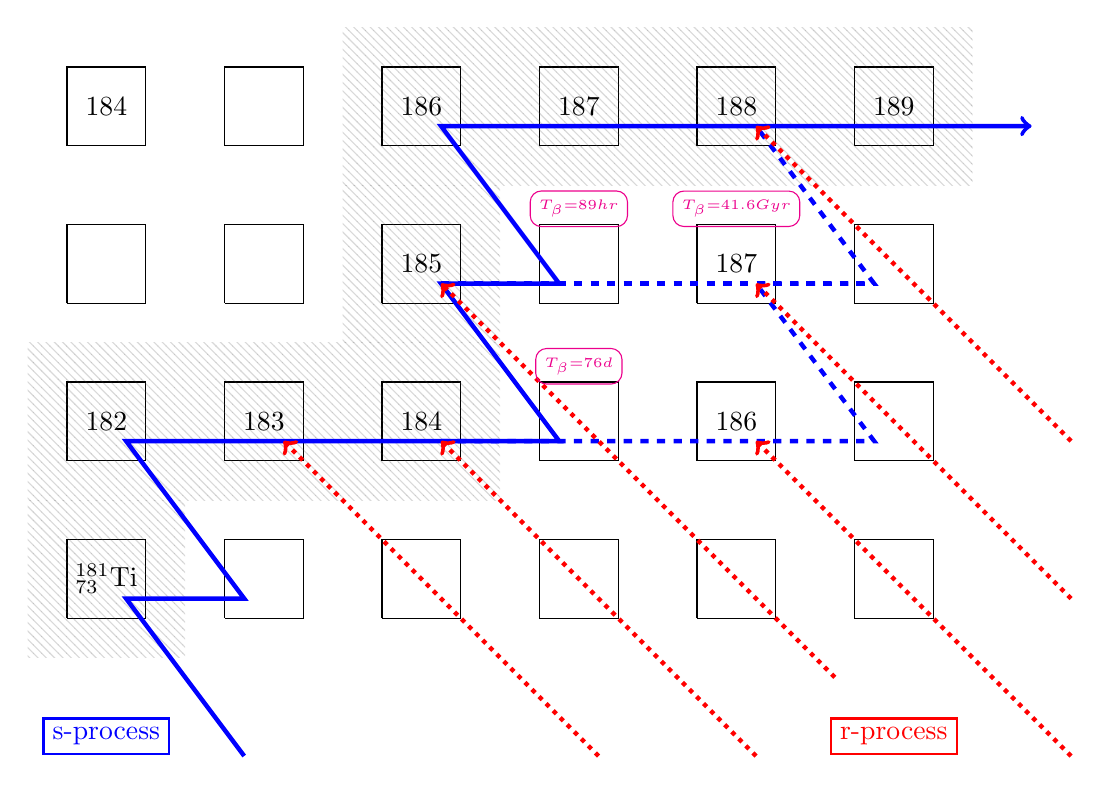
\begin{tikzpicture}
  %test in the middle
  %\draw (0,0) node {${}^{A+1}_{Z}$X};
  %\tikzsquare{0}{0}{\halfwidthnuclides}
  %Os-row on top of test
  \iffalse %old version
  \draw (-\distancenuclides,\distancenuclides) node {${}^{186}_{76}$Os};
  \tikzsquare{-\distancenuclides}{\distancenuclides}{\halfwidthnuclides}
  \draw (0,\distancenuclides) node {${}^{187}_{76}$Os};
  \tikzsquare{0}{\distancenuclides}{\halfwidthnuclides}
  \draw (\distancenuclides,\distancenuclides) node {${}^{188}_{76}$Os};
  \tikzsquare{\distancenuclides}{\distancenuclides}{\halfwidthnuclides}
  %stable Re-isotopes
  \draw (-\distancenuclides,0) node {${}^{185}_{75}$Re};
  \tikzsquare{-\distancenuclides}{0}{\halfwidthnuclides}
  \draw (\distancenuclides,0) node {${}^{187}_{75}$Re};
  \tikzsquare{\distancenuclides}{0}{\halfwidthnuclides}
  %W island of stability
  \draw (\distancenuclides,-\distancenuclides) node {${}^{186}_{74}$W};
  \tikzsquare{\distancenuclides}{-\distancenuclides}{\halfwidthnuclides}
  %shaded region of stability
  \fill[color=lightgray,opacity=0.1, pattern=north west lines, pattern color=darkgray]
  (-0.5\distancenuclides,-0.5\distancenuclides)
  rectangle (-1.5\distancenuclides,1.5\distancenuclides)
  rectangle (1.5\distancenuclides,0.5\distancenuclides)
  rectangle (0.5\distancenuclides,-1.5\distancenuclides);
  \fi

  %draw stable nuclei from clayton64 fig.1.
  %row1 - Os-184, blank, Os-186, Os-187, Os-188, Os-189
  \drawnuclide{-3\distancenuclides}{\distancenuclides}{\halfwidthnuclides}{\os{184}};
  \drawsquare{-2\distancenuclides}{\distancenuclides}{\halfwidthnuclides};
  \drawnuclide{-\distancenuclides}{\distancenuclides}{\halfwidthnuclides}{\os{186}};
  \drawnuclide{0}{\distancenuclides}{\halfwidthnuclides}{\os{187}};
  \drawnuclide{\distancenuclides}{\distancenuclides}{\halfwidthnuclides}{\os{188}};
  \drawnuclide{2\distancenuclides}{\distancenuclides}{\halfwidthnuclides}{\os{189}};
  %row2 - blank, blank, Re-185, blank, Re-187, blank
  \drawsquare{-3\distancenuclides}{0}{\halfwidthnuclides};
  \drawsquare{-2\distancenuclides}{0}{\halfwidthnuclides};
  \drawnuclide{-\distancenuclides}{0}{\halfwidthnuclides}{\re{185}};
  \drawsquare{0}{0}{\halfwidthnuclides};
  \drawnuclide{\distancenuclides}{0}{\halfwidthnuclides}{\re{187}};
  \drawsquare{2\distancenuclides}{0}{\halfwidthnuclides};
  %row3 - W-182, W-183, W-184, blank, W-186, blank
  \drawnuclide{-3\distancenuclides}{-\distancenuclides}{\halfwidthnuclides}{\w{182}};
  \drawnuclide{-2\distancenuclides}{-\distancenuclides}{\halfwidthnuclides}{\w{183}};
  \drawnuclide{-\distancenuclides}{-\distancenuclides}{\halfwidthnuclides}{\w{184}};
  \drawsquare{0}{-\distancenuclides}{\halfwidthnuclides};
  \drawnuclide{\distancenuclides}{-\distancenuclides}{\halfwidthnuclides}{\w{186}};
  \drawsquare{2\distancenuclides}{-\distancenuclides}{\halfwidthnuclides};
  %row4 - Ta-181, blank, blank, blank, blank, blank
  \drawnuclide{-3\distancenuclides}{-2\distancenuclides}{\halfwidthnuclides}{${}^{181}_{73}$Ti};
  \drawsquare{-2\distancenuclides}{-2\distancenuclides}{\halfwidthnuclides};
  \drawsquare{-\distancenuclides}{-2\distancenuclides}{\halfwidthnuclides};
  \drawsquare{0}{-2\distancenuclides}{\halfwidthnuclides};
  \drawsquare{\distancenuclides}{-2\distancenuclides}{\halfwidthnuclides};
  \drawsquare{2\distancenuclides}{-2\distancenuclides}{\halfwidthnuclides};

  %shaded region of stability
  \fillrectangle{-3\distancenuclides}{-2\distancenuclides}{2\halfwidthnuclides}; %Ta-181
  \fillrectangle{-3\distancenuclides}{-\distancenuclides}{2\halfwidthnuclides}; %W-182
  \fillrectangle{-2\distancenuclides}{-\distancenuclides}{2\halfwidthnuclides}; %W-183
  \fillrectangle{-\distancenuclides}{-\distancenuclides}{2\halfwidthnuclides}; %W-184
  \fillrectangle{-\distancenuclides}{0}{2\halfwidthnuclides}; %Re-185
  \fillrectangle{-\distancenuclides}{\distancenuclides}{2\halfwidthnuclides}; %Os-186
  \fillrectangle{0}{\distancenuclides}{2\halfwidthnuclides}; %Os-187
  \fillrectangle{\distancenuclides}{\distancenuclides}{2\halfwidthnuclides}; %Os-188
  \fillrectangle{2\distancenuclides}{\distancenuclides}{2\halfwidthnuclides}; %Os-189
  %\fillrectangle{\distancenuclides}{0}{2\halfwidthnuclides}; %Re-187
  %\fillrectangle{\distancenuclides}{-\distancenuclides}{2\halfwidthnuclides}; %W-186

  %draw s-process path
  \draw [ultra thick, ->, blue] (-2\distancenuclides-\offset,-3\distancenuclides-\offset)
  -- (-3\distancenuclides+\offset,-2\distancenuclides-\offset) -- (-2\distancenuclides-\offset,-2\distancenuclides-\offset)
  -- (-3\distancenuclides+\offset,-\distancenuclides-\offset) -- (0-\offset,-\distancenuclides-\offset)
  -- (-\distancenuclides+\offset,0-\offset) -- (0-\offset,0-\offset)
  -- (-\distancenuclides+\offset,\distancenuclides-\offset) -- (3\distancenuclides-\offset,\distancenuclides-\offset);
  %draw s-process branching point
  \draw [ultra thick, dashed, blue] (-\distancenuclides+\offset,-\distancenuclides-\offset)
  -- (2\distancenuclides-\offset,-\distancenuclides-\offset) -- (\distancenuclides+\offset,0-\offset)
  -- (2\distancenuclides-\offset,0-\offset) -- (\distancenuclides+\offset,\distancenuclides-\offset);
  \draw [ultra thick, dashed, blue] (-\distancenuclides+\offset,0-\offset)
  -- (2\distancenuclides-\offset,0-\offset);

  %draw r-process paths
  \draw [ultra thick, dotted, ->, red] (0+\offset,-3\distancenuclides-\offset)
  -- (-2\distancenuclides+\offset,-\distancenuclides-\offset);
  \draw [ultra thick, dotted, ->, red] (\distancenuclides+\offset,-3\distancenuclides-\offset)
  -- (-\distancenuclides+\offset,-\distancenuclides-\offset);
  \draw [ultra thick, dotted, ->, red] (1.5\distancenuclides+\offset,-2.5\distancenuclides-\offset)
  -- (-\distancenuclides+\offset,0-\offset);
  \draw [ultra thick, dotted, ->, red] (3\distancenuclides+\offset,-3\distancenuclides-\offset)
  -- (\distancenuclides+\offset,-\distancenuclides-\offset);
  \draw [ultra thick, dotted, ->, red] (3\distancenuclides+\offset,-2\distancenuclides-\offset)
  -- (\distancenuclides+\offset,0-\offset);
  \draw [ultra thick, dotted, ->, red] (3\distancenuclides+\offset,-\distancenuclides-\offset)
  -- (\distancenuclides+\offset,\distancenuclides-\offset);

  %add text
  \addtolength\offset{1.8\offset}
  \draw (-3\distancenuclides, -3\distancenuclides) node[thick, draw, blue] {s-process};
  \draw (2\distancenuclides, -3\distancenuclides) node[thick, draw, red] {r-process};
  \draw (0,0+\offset) node[draw=magenta, magenta, rounded corners] {${\scriptscriptstyle T_{\beta}=89hr}$}; %halflife of Re-186
  \draw (0,-\distancenuclides+\offset) node[draw=magenta, magenta, rounded corners] {${\scriptscriptstyle T_{\beta}=76d}$}; %halflife of W-185
  \draw (\distancenuclides,0+\offset) node[draw=magenta, magenta, rounded corners] {${\scriptscriptstyle T_{\beta}=41.6Gyr}$}; %halflife of Re-187
  \addtolength\offset{-1.8\offset}
\end{tikzpicture}
\caption[Chart of nuclides from \mycitetwo{clayton64}{fig.1} around A=187]{\label{tikz:nuclide-chart}
  Chart of nuclides around massnumber 187, adopted from \mycitetwo{clayton64}{fig.1}.
  The stable nuclei are denoted with their chemical symbols.
  The path of the s-process follows the valley of stability (shaded region), and is drawn as a blue solid line.
  Neutrons are absorbed during the s-process until and unstable isotope is reached, the unstable nuclide then \betadecay{s} to the higher isobars\footnote{the highest stable isobar means the nuclei with the same amount of nucleons and the highest amount of protons}.
  R-process nuclei are already very neutron-rich, and \betadecay{s} to the highest stable isobar.
  The path of the r-process is shown as red dotted lines.
  \w{185}, and also \re{186}, are potential branching points (), and can cause branched s-proces paths that are shown as blue dashed lines.
  The half-lifes of these potential branching point nuclei, as well as the half-life of \re{187}, are written in magenta over the nuclei.
}

    \caption{Adopted from \mycitetwo{clayton64}{fig.1}}
  \end{figure}
\end{frame}

\begin{frame}
  \frametitle{Analytical models of \re{187}-\os{187} cosmic clock}
  \begin{align}
    \frac{dN}{dt} &= -\lambda N \\
    \os{187}_{\astrosun} &= \os{187}_{s} + \os{187}_{p} + \os{187}_{c} \\
    \frac{d}{dt}\left[\os{187}_{c}\right] &= \lambda_\beta \re{187} \\
    \frac{d}{dt}\left[\re{187}\right] &= A(t) - \lambda_\beta \re{187} 
  \end{align}
  Using the analytical model from Clayton \mycite{clayton64}
  \begin{align}
    A(t) &= A_0e^{-\lambda_{r}t} \\
    f_{187} \equiv \frac{\os{187}_c}{\re{187}} &= \frac{\frac{\lambda_\beta}{\lambda_r} (1-e^{-\lambda_r t}) - (1-e^{-\lambda_\beta t})}{e^{-\lambda_{r}t}-e^{-\lambda_\beta t}}
  \end{align}
\end{frame}

\begin{frame}
  \frametitle{Observed isotope fraction from meteorites and solar atmosphere}
  \begin{align}
    \os{187}_{\astrosun}/\re{187}_{\astrosun} &= 0.226 \pm 0.0579 \quad \mycite{Shizuma05} \\ %f_{187}(t_{now}) = 
    \Delta t_{sos} &= 4.5682 \pm (4\times10^{-4}) Gyr \quad \mycite{bouvier10} \\
    T_{1/2} &= 41.577 \pm 0.12 Gyr \quad \mycite{snelling15} \\
    f_{187}(t_{sos}) &= 0.135 \pm 0.0323 %\os{187}_{\astrosun}/\re{187}_{\astrosun} 
  \end{align}
\end{frame}

%% \begin{frame}
%%   \frametitle{Formation of stellar systems in the Galaxy}
%%   \begin{itemize}
%%   \item Collapse of gas in giant molecular clouds
%%   \item Recycling of material from explosive events
%%   \item Inflow and outflow of gas from circumgalactic and extragalactic medium
%%   \end{itemize}
%% \end{frame}

\begin{frame}
  \frametitle{Chemical enrichment of galactic medium}
  \begin{figure}
    \centering
    \includegraphics[height=0.9\textheight]{\curdir{stellar_recycling.png}}
  \end{figure}
\end{frame}

\begin{frame}
  \frametitle{Explosive events}
  \begin{itemize}
  \item Asymptotic giant branch stars (not really explosive)
  \item Core collapse supernovae
  \item Type 1a supernovae
  \item Neutron star mergers
  \end{itemize}
\end{frame}

\begin{frame}
  \frametitle{Eris simulation}
  \begin{minipage}{0.45\linewidth}
    \begin{figure}
      \centering
      \includegraphics[width=\linewidth]{../thesis/img/eris_map_guedes11_fig2.png}
      \caption{credit: Guedes et al. (2011) \mycitetwo{guedes11}{fig.2}}
    \end{figure}
  \end{minipage}
  \hfill
  \begin{minipage}{0.45\linewidth}
    \begin{itemize}
    \item Smoothed particle hydrodynamics simulation \mycite{guedes11}
    \item 3D 
    \item 18.6 million particles
    \item Postprocessing to add rapid neutron capture elements from neutron star mergers \mycite{shen15}
    \end{itemize}
  \end{minipage}
\end{frame}

\begin{frame}
  \frametitle{Omega semianalytical model \mycite{cote16a}}
  \begin{itemize}
  \item SFR + timestep $\rightarrow$ stellar mass formed
  \item stellar mass formed $\rightarrow$ stellar population
  \item stellar population + yield tables + delay-time $\rightarrow$ isotopic yields recycled into ISM + remnant
  \item remnants $\rightarrow$ secondary events
  \end{itemize}
\end{frame}

\begin{frame}
  \centering
  \textbf{
    \Large
    \mytitle
  }
\end{frame}
